\section{Diseño-experimental}
\begin{frame}
    \frametitle{Diseño experimental}
    \vspace*{2mm}
    \textbf{\large Diseño cuasi-experimental}\\[5mm]
    
    \begin{itemize}[columns=2]
	    \item Temperatura de entrada del agua
	    \item Presión atmosférica
	    \item Temperatura ambiente
	    \item Nubosidad
	    \item Velocidad de viento
	    \item Hora del día
	    \item Irradiación solar promedio
	    \item Temperatura de salida del agua
	    \item Temperatura del recibidor solar
	    \item Caudal de agua
	    \item Propiedades fisicoquímicas del agua
    \end{itemize}
\end{frame}

	\subsection{Grupos de estudio}

	\begin{frame}
	    \frametitle{Grupos de estudio}
	    \vspace*{2mm}
	    \textbf{\large Agua}\\[5mm]  
	    
	    Las muestras de agua se seleccionaron guiándose en la clasificación propuesta por la \acrfull{wqa}. Se proponen 3 grupos para evaluar los casos límite y promedio de la salinidad del agua de mar.
	      
	    \begin{longtblr}[
			caption = {Grupo de control del agua de mar},
			label = {table:grupo-control-agua}
		]{
			colspec = {X[c] X[2, c]},
			hlines,
			vlines,
			width = 0.5\linewidth,
			rowhead = 1,
			row{odd} = {bg=tablerowblue},
			row{1} = {
				bg = tabletitleblue,
				fg=white,
				font = \bfseries,
				halign=c
			},
			rows={m}
		}
			Muestra & Salinidad (\unit{\mg\per\litre})\\
			1 & \num{30000}\\
			2 & \num{35000}\\
			3 & \num{40000}
		\end{longtblr}
	\end{frame}
	
	\begin{frame}
	    \frametitle{Lugar físico de experimentación}
	    \vspace*{2mm}
	    
	    Unidad Profesional Interdisciplinaria en Ingeniería y Tecnologías Avanzadas ubicada en la Ciudad de México.
			
			\begin{longtblr}[
				caption = {Grupo de control del agua de mar},
				label = {table:grupo-control-fisico}
			]{
				colspec = {X[c] *{3}{c}},
				hlines,
				vlines,
				width = 0.8\linewidth,
				rowhead = 1,
				row{odd} = {bg=tablerowblue},
				row{1} = {
					bg = tabletitleblue,
					fg=white,
					font = \bfseries,
					halign=c
				},
				rows={m}
			}
				Zona & Longitud & Latitud & Altitud\\
				Ciudad de México, México
					& \ang{-99;07;32}
					& \ang{19;30;38}
					& \qty{2241}{\m}
			\end{longtblr}
	    
	\end{frame}
	
	\subsection{Problemas asociados a la destilación solar}
	\begin{frame}
	    \frametitle{Problemas asociados a la destilación solar}
	    \vspace*{2mm}
	    
	    \textbf{\large Problemas identificados}\\[5mm]
	    
	    \begin{columns}
	    		\begin{column}{0.5\linewidth}
	    			\begin{figure}
	    				\includegraphics[
		    				width=\linewidth
	    				]{Desarrollo/condensación.jpg}
	    				\caption{Transmitancia afectada por la condensación}
	    			\end{figure}
		    \end{column}
		    \begin{column}{0.5\linewidth}
		    		\begin{figure}
	    				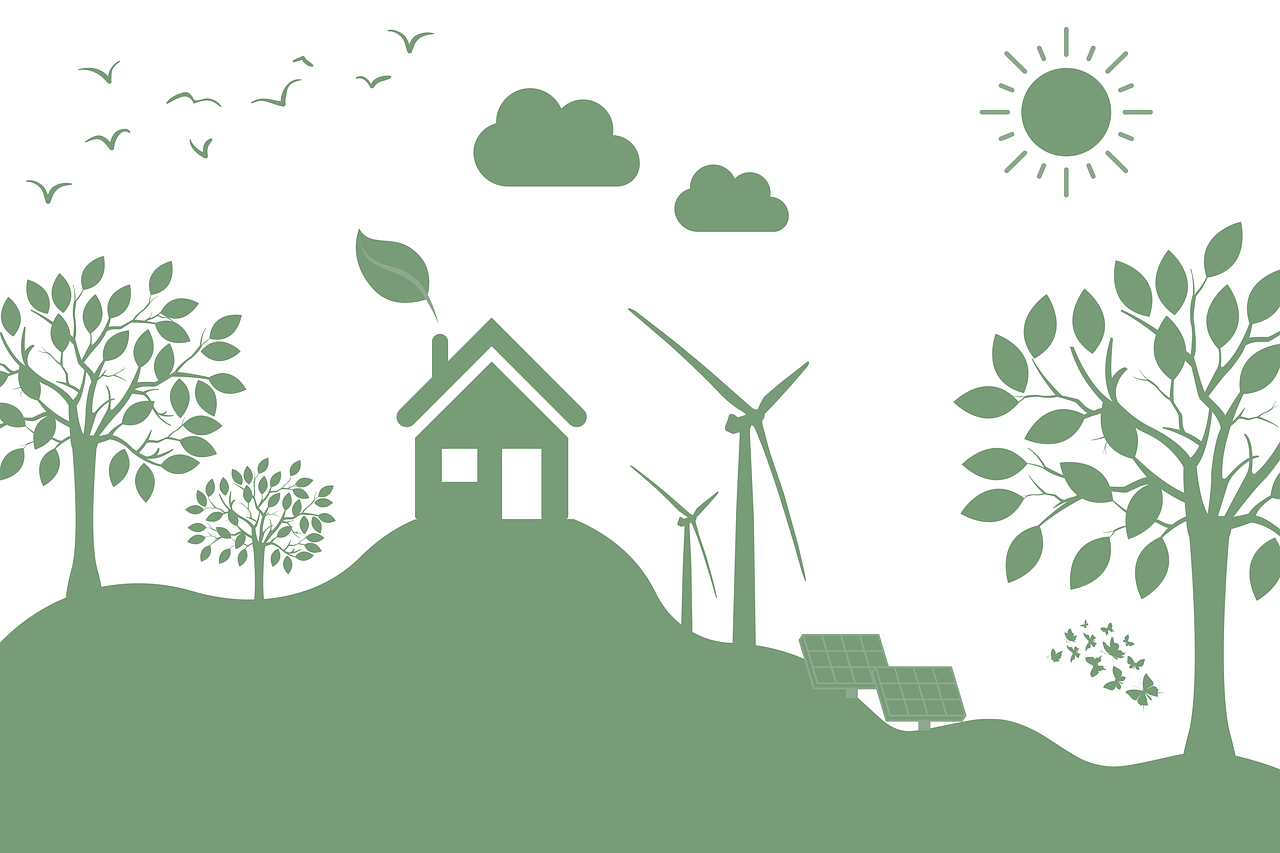
\includegraphics[
		    				width=\linewidth
	    				]{Desarrollo/intermitencia.png}
	    				\caption{Forma de energía discontinua}
	    			\end{figure}
		    \end{column}
	    \end{columns}
	\end{frame}
		
	\subsection{Configuración experimental}
	\begin{frame}
	    \frametitle{Configuración experimental}
	    \vspace*{2mm}
	    
	    \textbf{\large Análisis de las variables mencionadas}\\[5mm]
	    
	    \begin{columns}
	    		\begin{column}{0.6\textwidth}
	    			Para definir los criterios de operación sobre los cuales se espera que opere en pruebas el sistema, se realizó un análisis de datos de las variables climáticas propuestas. Los datos utilizados fueron obtenidos de \textit{NASA Langley Research Center (LaRC) POWER Project} financiado por el Programa de Ciencias de la Tierra/Ciencias Aplicadas de la NASA
		    \end{column}
		    \begin{column}{0.4\textwidth}
			    \centering
		    		\begin{figure}
		    			\centering
		    			
\includegraphics[width=\linewidth]{julia.png}
		    			\caption{Lenguaje de programación empleado para el análisis de datos}
		    			\label{fig:julia}
		    		\end{figure}
		    \end{column}
	    \end{columns}
	\end{frame}
	
	\begin{frame}
	    \frametitle{Configuración experimental}
	    \vspace*{2mm}
	    
	    \textbf{\large Irradiación solar de onda corta}\\[5mm]
	    
	    \begin{columns}
		    \begin{column}{0.5\textwidth}
		    		Del análisis de datos se obtuvo:
			    \begin{itemize}
			    		\item Mínimo de operación \qty{400}{\watt\per\m\tothe{2}}
			    		\item Máximo de operación \qty{900}{\watt\per\m\tothe{2}}
			    		\item Operación general \qty{650}{\watt\per\m\tothe{2}}
			    		\item Inicio de irradiación a las 7:00 a.m.
			    		\item Fin de irradiación a las 6:00 p.m.
			    \end{itemize}
		    \end{column}
		    \begin{column}{0.5\textwidth}
			    \centering
		    		\begin{figure}
		    			\centering
		    			\only<1>{
		    				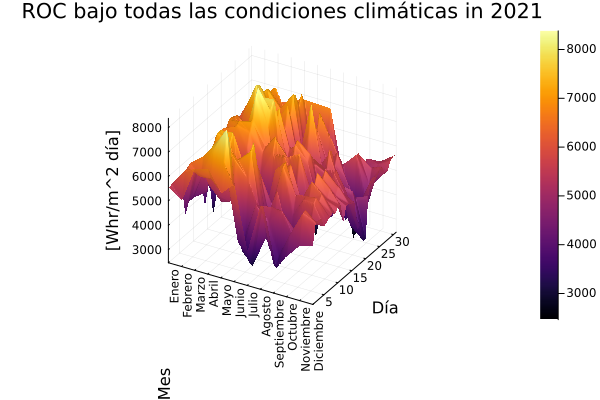
\includegraphics[
		    					width=\linewidth
			    			]{Resultados/DataAnalysis/ALLSKY_SFC_SW_DWN_surface_2021_3d.png}
		    			}
		    			\only<2>{
		    				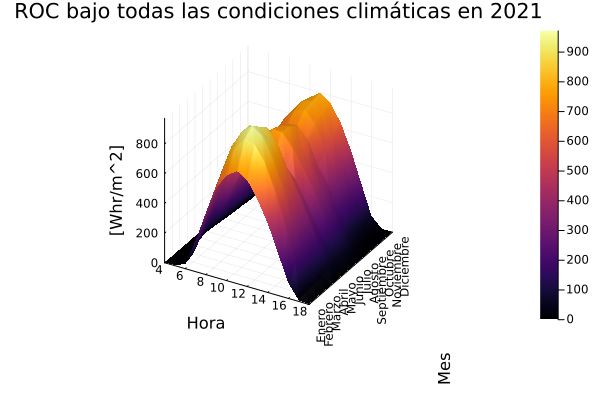
\includegraphics[
			    				width=\linewidth
			    			]{Resultados/DataAnalysis/ALLSKY_SFC_SW_DWN_3d_mean_2021.png}
		    			}
		    			\caption{Radiación de onda corta 2021}
		    			\label{fig:ALLSKY_SFC_SW_DWN_surface_2021_3d}
		    		\end{figure}
		    \end{column}
	    \end{columns}
	\end{frame}
	
	\begin{frame}
	    \frametitle{Configuración experimental}
	    \vspace*{2mm}
	    
	    \textbf{\large Temperatura ambiente}\\[5mm]
	    
	    \begin{columns}
			\begin{column}{0.5\textwidth}
				Del análisis de datos se obtuvo:
			    \begin{itemize}
			    		\item Mínimo de temperatura \qty{13}{\degreeCelsius}
			    		\item Máximo de temperatura \qty{29}{\degreeCelsius}
			    		\item Temperatura de entrada del agua \qty{15.5}{\degreeCelsius}
			    \end{itemize}
		    \end{column}
		    \begin{column}{0.5\textwidth}
			    \centering
		    		\begin{figure}
		    			\centering
		    			\includegraphics[
		    				width=\linewidth
		    			]{Resultados/DataAnalysis/Temperatura-por-hora-en-2022-Ciudad-de-México.png}
		    			\caption{Gráfico obtenido de \href{https://es.weatherspark.com/y/5674/Clima-promedio-en-Ciudad-de-México-México-durante-todo-el-año}{\textcopyright WeatherSpark.com}}
		    			\label{fig:Temperatura-por-hora-en-2022-Ciudad-de-México}
		    		\end{figure}
		    \end{column}
	    \end{columns}
	\end{frame}
	
	\begin{frame}
	    \frametitle{Configuración experimental}
	    \vspace*{2mm}
	    
	    \textbf{\large Presión atmosférica}\\[5mm]
	    
	    \begin{columns}
		    \begin{column}{0.5\textwidth}
		    		Del análisis de datos se obtuvo:
			    \begin{itemize}
			    		\item Variación mínima
			    		\item Presión de \qtyrange{74.45}{74.80}{\kilo\pascal}
			    		\item Se calculó cambio de fase del agua de mar a \qty{94.7}{\degreeCelsius}
			    \end{itemize}
		    \end{column}
		    \begin{column}{0.5\textwidth}
			    \centering
		    		\begin{figure}
		    			\centering
		    			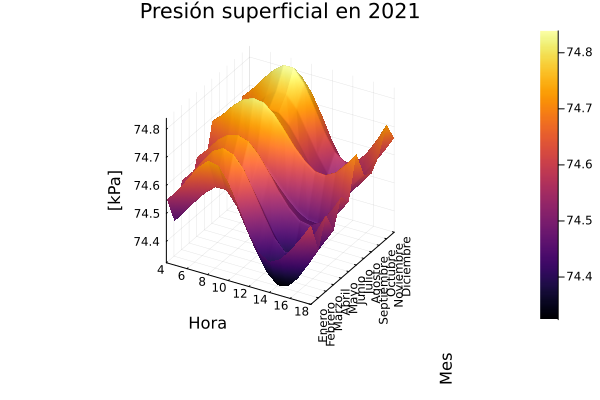
\includegraphics[
		    				width=\linewidth
		    			]{Resultados/DataAnalysis/PS_3d_mean_2021.png}
		    			\caption{Presión promedio por hora durante 2021}
		    			\label{fig:PS_3d_mean_2021}
		    		\end{figure}
		    \end{column}
	    \end{columns}
	\end{frame}
	
	\begin{frame}
	    \frametitle{Configuración experimental}
	    \vspace*{2mm}
	    
	    \textbf{\large Velocidad de viento}\\[5mm]
	    \begin{columns}
		    \begin{column}{0.5\textwidth}
		    		Del análisis de datos se obtuvo:
			    \begin{itemize}
			    		\item Variación impredecible
			    		\item Velocidad de \qtyrange{0.50}{2.00}{\m\per\s}
			    \end{itemize}
		    \end{column}
		    \begin{column}{0.5\textwidth}
			    \centering
		    		\begin{figure}
		    			\centering
		    			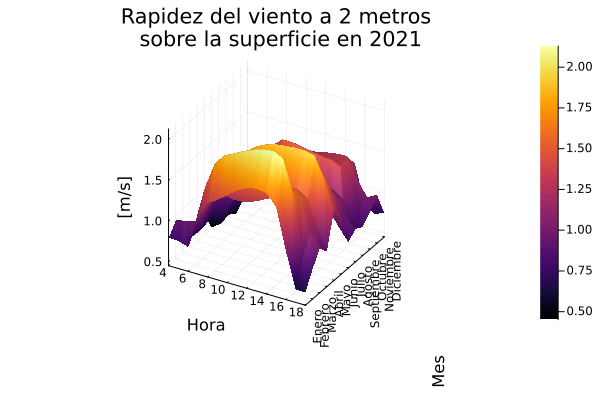
\includegraphics[
		    				width=\linewidth
		    			]{Resultados/DataAnalysis/WS2M_3d_mean_2021.png}
		    			\caption{Rapidez promedio del viento durante 2021}
		    			\label{fig:WS2M_3d_mean_2021}
		    		\end{figure}
		    \end{column}
	    \end{columns}
	\end{frame}
	
	\begin{frame}
	    \frametitle{Elemento óptico de concentración}
	    \vspace*{2mm}
	    
	    \begin{longtblr}[
				caption = {Modelos y características de los concentradores solares},
				label = {table:fresnel-lenses-models}
			]{
				colspec = {*{2}{X[1.5]} *{2}{X} X[3] *{2}{X}},
				hlines,
				vlines,
				width = \linewidth,
				rowhead = 2,
				row{odd[3]} = {bg=tablerowblue},
				row{1,2} = {
					bg = tabletitleblue,
					fg=white,
					font = \bfseries,
					halign=c
				},
				rows={
					halign = c,
					valign = m,
					font=\small
				}
			}
				Modelo & Longitud focal & Ancho & Largo & Material & Grosor & Tamaño de ranura\\
				--- & mm & mm & mm & --- & mm & mm\\
				CP220-280
					& \num{220}
					& \num{280}
					& \num{280}
					& PMMA: \acrshort{pvuvc}
					& \num{5}
					& \num{0.5}\\
				CP330-280
					& \num{330}
					& \num{280}
					& \num{280}
					& PMMA: \acrshort{pvuvc}
					& \num{5}
					& \num{0.5}\\
				CP350-300 
					& \num{350}
					& \num{310}
					& \num{310}
					& PMMA: \acrshort{pvuvc}
					& \num{5}
					& \num{0.5}\\
				CP350-330 
					& \num{350}
					& \num{340}
					& \num{340}
					& PMMA: \acrshort{pvuvc}
					& \num{5}
					& \num{0.5}
			\end{longtblr}
			
			Se halla en su hoja técnica que el PMMA \acrshort{pvuvc} tiene una transmitancia igual a \percent{92.65}.
	\end{frame}
	
	\begin{frame}
	    \frametitle{Pérdidas por transmisión}
	    \vspace*{2mm}
	    
	    La radiación que podría concentrar efectivamente esta lente de Fresnel sobre el recibidor solar usando las asunciones generales es de \qty{43.51}{\watt}.
	    
	    \begin{equation}\label{equ:radiación-concentrada}
			\dot{Q}_{\text{absorbedor}} = \alpha \tau I_{\text{Sol}} A_\text{Fresnel}
		\end{equation}
		
		Con base en esto se definió un caudal de \qty{8.26}{\milli\litre\per\minute}.
		
	\end{frame}